\section{14. Financial Plan \& Break-Even Analysis}
\subsection{Revenue Projections}
\begin{tabular}{|c|c|c|c|c|}
\hline
\textbf{Year} & \textbf{Pay-Per-Use} & \textbf{Subscriptions} & \textbf{Installations} & \textbf{Total Revenue} \\
\hline
1 & €805k & €696k & €750k & €2.25M \\
\hline
2 & €1.6M & €2.2M & €1.2M & €5M \\
\hline
3 & €2.8M & €3.9M & €2M & €8.7M \\
\hline
\end{tabular}

\subsection{Expense Breakdown}
\begin{tabular}{|l|r|r|}
\hline
\textbf{Category} & \textbf{Fixed (€)} & \textbf{Variable (€)} \\
\hline
Salaries & 400k & – \\
\hline
Maintenance & 100k & €200/station/month \\
\hline
Marketing & 150k & – \\
\hline
Energy & – & €0.10/kWh \\
\hline
\end{tabular}

\subsection{Break-Even Analysis}
\begin{itemize}
    \item \textbf{Fixed Costs:} €1.2M/year.
    \item \textbf{Contribution Margin/Charger:} €48k revenue – €24k variable costs = €24k.
    \item \textbf{Break-Even Point:} €1.2M ÷ €24k = 50 chargers (33\% utilization).
\end{itemize}

\subsection{Expense Breakdown}
\begin{figure}[h!]
    \centering
    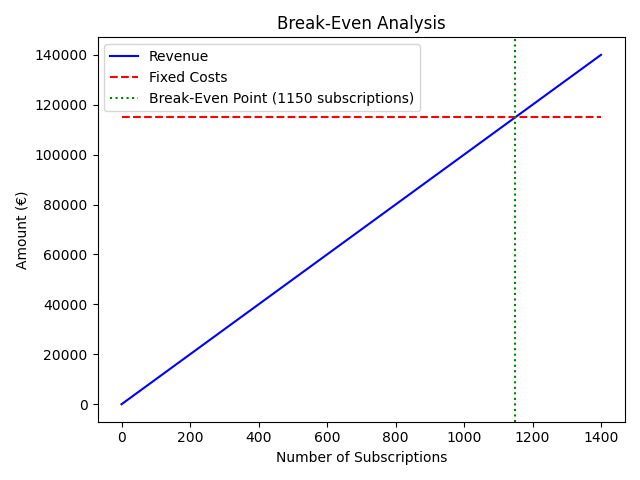
\includegraphics[width=0.8\textwidth]{images/Break Even.png}
    \caption{Expense breakdown showing fixed and variable costs.}
    \label{fig:expense_breakdown}
\end{figure}



\subsection{Conclusion}
By 2027, DynoCharge aims to achieve €12M in revenue and capture a 25\% market share in Europe’s fast-charging segment. Our focus on speed, sustainability, and strategic partnerships positions us to lead the transition to zero-emission mobility.
